\documentclass[11pt,oneside,a4paper,numbers=enddot]{report} % scrreprt
\usepackage{thema}

\begin{document}
\Pre

\chapter{Inleiding}
*Fill with content*

\chapter{Weekopdracht 1}

Wij verbinden bedrijven
Wij laten bedrijven samenwerken
Community van bedrijven
Wij introduceren bedrijven aan elkaar
Matchmaker voor bedrijfrelaties
Om bedrijven makkelijk met elkaar in contact te brengen voor het delen van services.
door middel van delen van services

\section{Servicemarkt}

\subsection{Missie}
Het platform voor bedrijfsservices zijn.

\subsection{Visie}
Wij geven bedrijven de kans om elkaar te ontmoeten, zodat ze elkaar kunnen helpen. \\
Wij laten hen in contact komen, zodat ze elkaars services kunnen benutten.

\subsection{Doelen}

\begin{itemize}
\item
  Wij streven ernaar om bekend te worden als een betrouwbare plaats om services aan te bieden.
\item
  Een mooie website opzetten waar bedrijven makkelijk gebruik van kunnen maken
\item
  Wij willen het kortste lijntje tussen bedrijven zijn. (Een verbindingspunt zijn voor bedrijven)
\item
  
\end{itemize}

\subsection{Omschrijving}
Een belangrijk punt om op te doelen is, dat wij als bedrijf veel contact hebben met bedrijven, wat dit leidt tot goede communicatie, 
maar ook dat wij kunnen anticiperen op verschillende situaties, wat ook weer leidt tot een goede werkende website met verschillende aangebode services van allerlei bedrijven, waardoor wij groeien als bedrijf en lijdt tot een populair platform voor bedrijven.

*is de communicatie met veel bedrijven. ook hierdoor wordt onze naam bekend waardoor*


bespreken over hoe en wat de situaties zijn en wat hun belangen zi


\chapter{Weekopdracht 2}

\section{SWOT van Jan Sietze}

\subsection{Strengths}

\begin{itemize}
\item
  Systeembeheerder geweest
\item
  Leert graag nieuwe vaardigheden
\item
  Programmeerervaring
\item
  Design ervaring
\item
  Structureel
\end{itemize}

\subsection{Weaknesses}

\begin{itemize}
\item
  Wordt snel moe
\item
  Snel overwerkt
\item
  Houdt niet van authoritaire relaties
\item
  Heeft structuur en duidelijkheid nodig
\item
  Slecht korte-termijn geheugen
\end{itemize}

\subsection{Opportunities}

\begin{itemize}
\item
  
\item
   
\item
  IT-markt is groot en groeit
\item
  IT is gestructureerd en logisch
\item
  ICT is erg breed en overal nodig
\end{itemize}

\subsection{Threats}

\begin{itemize}
\item
  Veel competitie in ICT voor sommige taken/banen
\item
  Groot aantal ICT-studenten
\item
  Hoge werkdruk op school
\item
  IT veranderd snel
\item
  Veel dingen moeten zeker goed gebeuren
  
\end{itemize}

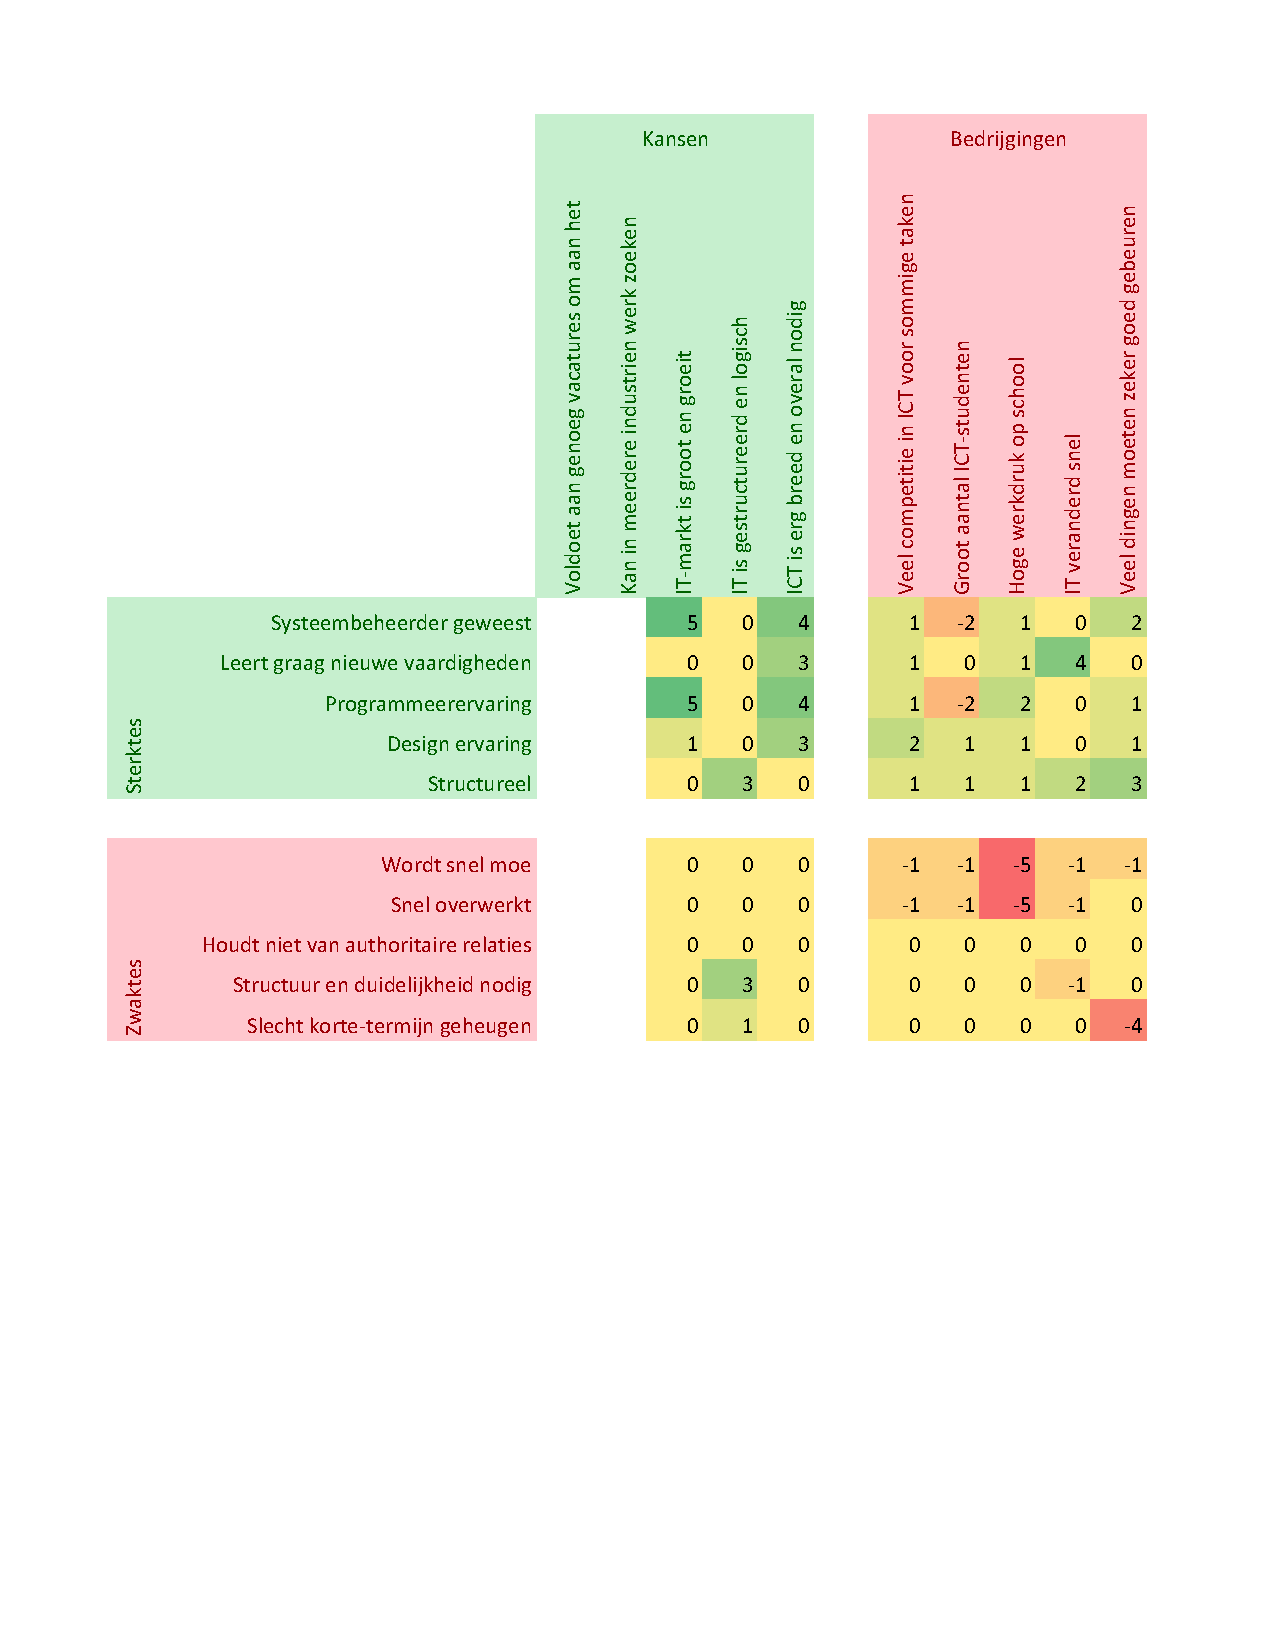
\includegraphics[width=\textwidth]{other/Swot-matrix-Jan}

\section{SWOT van Niek}

\subsection{Sterktes}

\begin{itemize}
\item
  Enthousiast
\item
  Sociaal
\item
  Redelijk creatief
\item
  Gemotiveerd om nieuwe dingen te leren
\item
  Behulpzaam
\item
  Goed in communicatie
\item
  Achtergrond van systeembeheerder
\item
  Ondersteunen van mensen
\item
  Het documenteren van projecten/informatie
\item
  Inspringen bij bepaalde activiteiten
\item
  Organiseren van informatie
\end{itemize}

\subsection{Zwaktes}

\begin{itemize}
\item
  Soms duidelijkheid nodig om zeker van de zaak te zijn
\item
  Soms te veel dingen oppakken
  binnen bepaalde activiteiten
  en dan het werk waarmee je bezig was dan vergeet
\item
  Soms te veel vragen stellen over bepaald iets,
  wanneer het al goed is of
  wanneer je de keuze moet maken over iets
\end{itemize}
  
\subsection{Kansen}

\begin{itemize}
\item
  Er is best veel vraag binnen de ICT-sector
\item
  ICT-markt groeit
\item
  Bedrijven doen meer met ICT
\end{itemize}

\subsection{Bedreigingen}

\begin{itemize}
\item
  Aantal ICT studenten neemt toe
\item
  Er zijn te hoge verwachtingen vanuit bedrijven
  terwijl mensen met een lager niveau hetzelfde zouden kunnen behalen
  als mensen met een hoog niveau
\item
  ICT levert meer werk op,
  maar kan veroorzaken dat er minder personeel nodig is binnen bedrijven.
\end{itemize}

\section{SWOT Annelies van Joost}

\subsection{Sterktes}
\begin{itemize}
\item Enthousiast
\item Optimistisch
\item Creatief
\item Gemotiveerd om nieuwe dingen te leren
\item Ondersteunend
\item Goed in communicatie
\item Goed economisch verstand
\item Redelijk in ICT
\end{itemize}

\subsection{Zwaktes}
\begin{itemize}  
\item Veel moe
\item Aan de luie kant
\item Snel afgeleid
\item Vergeet snel dingen
\item Niet geweldig met afspraken maken
\item Duidelijkheid nodig
\end{itemize}

\subsection{Kansen}
\begin{itemize}
\item Er is vraag naar goede communicatie
\item Economische kennis is nodig
\item ICT markt is groot en groeit
\item Gemotiveerd om in meerder bedrijfstakken aan de slag te gaan
\end{itemize}

\subsection{Bedreigingen}
\begin{itemize}
\item Toenemend aantal ICT studenten
\item Redelijk hoge werkdruk
\item ICT kennis niet de beste van de besten
\end{itemize}

\section{Zelf SWOT-Analyse Tjibbe Masselink}
\subsection{Strengths}
\begin{itemize}
\item
  Breed denkend
\item
  Havo-diploma en vmbo-diploma
\item
  Presenteer skills
\end{itemize}

\subsection{Weaknesses}
\begin{itemize}
\item
  Afwezig
\item
  Heeft een prikkel nodig
\item
  Werk te verrichten
\item
  Snel en veel afgeleid
\item
  Te laat regelmatig
\end{itemize}

\subsection{Opportunities}
\begin{itemize}
\item
  Kan veel inbreng geven in onderwerpen
\end{itemize}

\subsection{Threats}
\begin{itemize}
\item
  Druk op school
\item
  Stress
\item
  Motivatie
\item
  Deadline werker
\item
  Slechtste van de klas kunnen wezen
\end{itemize}

\section{Swot-Analyse bedrijf}

\subsection{Sterktes}
\begin{itemize}
\item {\bf Een origineel bedrijf} \\
  Wij geloven dat wij een origineel idee hebben en staan hier met erg veel motivatie achter.
\item {\bf Goede communicatie} \\
  Als bedrijf is het voor ons belangrijk om bereikbaar te zijn voor mensen die gebruik maken van onze faciliteiten, vandaar dat wij altijd klaar willen staan om te helpen.
\item {\bf Een helpende hand} \\
  Wij willen kleine bedrijven helpen opstarten door hun makkelijk te vinden te maken. Zo proberen wij de industrie en markt van die bepaalde onderneming te verbreden.
\item {\bf Duidelijkheid} \\
  Als bedrijf willen wij duidelijke regels opstellen voor het gebruikmaken van de faciliteiten en het samenwerken tussen ondernemingen. Als deze regels niet worden nageleefd zullen wij als bedrijf hard optreden. Zo creëren wij een veilige en duidelijke omgeving voor alle betrokken ondernemingen.
\item {\bf Uitgebreide marktkeuze} \\
  Wij proberen om bedrijven van elke bedrijvensector gebruik te laten maken van onze service, zo willen wij een gigantische keuze aan bedrijven aanbieden voor wat voor markt dan ook.
\end{itemize}
\subsection{Zwaktes}
\begin{itemize}
\item {\bf Simpel idee} \\
  Hoewel het idee origineel is, kan het zo door anderen overgenomen worden. Het creëren van dit bepaalde netwerk is niet heel erg lastig. Het zal waarschijnlijk om kwaliteit van de site, betrouwbaarheid en naambekendheid gaan.
\item {\bf Lastig te onderhouden naarmate de groei van het bedrijf.} \\
  Hoe groter ons bedrijf wordt en hoe meer bedrijven er gebruik van gaan maken, hoe moeilijker het  wordt om elke handeling aandachtig te bestuderen en om te kijken of er wel goed gehandeld is. Bovendien moeten bedrijven die contact opnemen met onze hulpservice ook goed geholpen kunnen worden, wij willen wachtrijen voorkomen.
\item {\bf Geen gigantisch winstgevend bedrijf} \\
  Het meeste geld zal via reclames op de websites en via een klein tarief voor de bedrijven voor het gebruik van onze service zijn. Of dit een dikke winst zal geven is nog erg onduidelijk, maar als alleen website zal dit waarschijnlijk niet het geval zijn.
\end{itemize}
\subsection{Kansen}
\begin{itemize}
\item {\bf Kleine bedrijven} \\
  Wij kunnen de kleinere bedrijven zoals zzp’ers helpen met opstarten door hun naam op onze sites te zetten en hun een platform te geven waarop zij zichzelf kunnen neerzetten als de juiste keuze. Zo zullen deze ondernemingen sneller in contact kunnen komen met grote bedrijven en zal hun naambekendheid een flinke boost krijgen.
\item {\bf Snelle oplossingen gezocht} \\
  Als een bedrijf een probleem heeft wat snel opgelost moet worden zal onze site binnen een paar clicks zoveel mogelijk keuze aanbieden als oplossing. Wij willen een onpartijdige lijst zo snel mogelijk aanbieden met duidelijke info zodat er snel een keuze gemaakt kan worden.
\end{itemize}

\subsection{Bedreigingen}
\begin{itemize}
\item {\bf Een rivaal} \\
  Wanneer een ander bedrijf probeert een soortgelijke service aan te bieden, moeten wij ervoor zorgen dat wij de beste onderneming blijven die deze service aanbiedt. Dit kan erg lastig zijn.
\item {\bf Teveel klachten en hulp gevraagd} \\
  Als ons bedrijf hard groeit kan het lastig worden om orde te houden wanneer elke dag meerdere klachten worden ingezonden. Om dit te hanteren zijn veel werknemers nodig met mogelijk veel inspanning. 
\item {\bf Slechte naam} \\
  Wanneer een bedrijf een slechte ervaring heeft met betrekking tot de samenwerking met een ander bedrijf, kunnen zij de schuld mede geven aan ons, omdat wij dit bedrijf aan hun hebben aangeboden. Wij moeten dit voorkomen door een oplossing te bieden en duidelijk te maken dat niet alles in onze handen ligt, bijvoorbeeld hoe een bedrijf presteert.
\end{itemize}
\chapter{Opdracht week 4}

\section{Toepassing 1}

Als eerste werdt er natuurlijk gedacht aan het originele idee,
een website waarop services gedeeld en ingehuurd worden.

\subsection{Relatie SWOT}
{\bf Hoe zijn we op dit idee gekomen, hoe is dit gerelateerd}

\subsection{Uitbreidingsplan}

\subsubsection{Doel}
{\bf Bedoeling met het systeem, welke partijen hebben er mee te maken}

\subsubsection{Impact}
{\bf Wat is er nodig, wat gebeurt er met het bedrijf}

\subsubsection{Omschrijving}
{\bf Systeemontwerpen, wireframes, designs}

\section{Toepassing 2}

Een app zou eenzelfde soort functie kunnen leveren,
maar zal andere mensen aantrekken.
Een hypothese zou kunnen zijn dat een app het gemak verhoogd
en dus de markt groter maakt,
met een breder scala aan mensen.

\subsection{Relatie SWOT}
{\bf Hoe zijn we op dit idee gekomen, hoe is dit gerelateerd}

\subsection{Uitbreidingsplan}

\subsubsection{Doel}
{\bf Bedoeling met het systeem, welke partijen hebben er mee te maken}

\subsubsection{Impact}
{\bf Wat is er nodig, wat gebeurt er met het bedrijf}

\subsubsection{Omschrijving}
{\bf Systeemontwerpen, wireframes, designs}

\section{Toepassing 3}

\subsection{Relatie SWOT}
{\bf Hoe zijn we op dit idee gekomen, hoe is dit gerelateerd}

\subsection{Uitbreidingsplan}

\subsubsection{Doel}
{\bf Bedoeling met het systeem, welke partijen hebben er mee te maken}

\subsubsection{Impact}
{\bf Wat is er nodig, wat gebeurt er met het bedrijf}

\subsubsection{Omschrijving}
{\bf Systeemontwerpen, wireframes, designs}



\chapter{MOVE THIS}
\section{Wat is er benodigd}

Het doel is een bedrijf te starten, daarvoor moet je eerst naar de KvK.
Voordat je naar de KvK gaat, moet je beslissen onder welk rechtsvorm je bedrijf valt.
Dit beslis je door... 

Bij de KvK moet je verschillende dingen opleveren waaronder:

\begin{enumerate}

\item
  een unieke bedrijfsnaam (mogelijk meerdere)
\item
  50 euro voor inschrijving
\item
  Vestigingsplaats
  + adres
  + contactgegevens
\item
  Bedrag startkapitaal
\item
  Omschrijving bedrijfs- activiteiten,
  diensten en/of
  producten
\item
  Als er meerdere zijn de belangrijkste
\item
  Of je producten aan consumenten verkoopt,
  en waar
  (via internet,
  de kelder of winkelpand)
\item
  Of er producten worden ge- importeerd/exporteerd
\item
  Hoeveel mensen er zullen werken
  (full-time of part-time)
\item
  Hoeveel vennoten er zijn,
  hoe het bedrijf verdeelt is over deze personen,
  of er een vennootschapsakte is,
  etc.
  
\end{enumerate}

Bron: \cite{kvk}

\section{Wat wij gaan doen}

Wat wij dus gaan doen is het volgende:

\begin{itemize}
\item
  Kiezen wat we gaan doen als bedrijf
  -- Brainstormen
  -- Onderzoek doen
  -- Keuze vastleggen
  -- bovenstaande documenteren (Plan van Aanpak)
\item
  Bedrijfsnaam kiezen
  -- Controleren dat deze uniek is.
\item
  Beslissen hoeveel werknemers en
  hoeveel vennoten er initieel zullen zijn
\item
  Kiezen waar het bedrijf wordt gevestigd
\item
  Financieel plan maken
  -- Bedenken waar we geld verdienen (verdienmodel) en verliezen
  -- Gaan onderzoeken en bereken hoeveel deze aantallen zijn
  -- Lening
  --- Berekenen hoeveel te lenen
  --- Lening aanvragen bij bank
\item
  Inschrijven bij KvK -- Belastingdienst wordt `automatisch' geregeld
  wanneer ingeschreven bij KvK
\end{itemize}

\begin{thebibliography}{1}

\bibitem{kvk} \href{https://www.kvk.nl}{kvk.nl} {\em Website van de Kamer van Koophandel}  2018.

\end{thebibliography}

\end{document}
%%% Local Variables:
%%% mode: latex
%%% TeX-master: t
%%% End:
